% \documentclass[reprint, amsmath,amssymb,aps,pra]{revtex4-2}
\documentclass[11pt,reqno]{amsart}

\usepackage[pdfborder={0 0 0.5 [3 2]}, plainpages=false]{hyperref}%
\usepackage[left=1in,right=1in,top=1in,bottom=1in]{geometry}%
% \usepackage[shortalphabetic]{amsrefs}%
\usepackage{amsmath}
\usepackage{enumerate}
% \usepackage{enumitem}
\usepackage{amssymb}                
\usepackage{amsmath}                
\usepackage{amsfonts}
\usepackage{amsthm}
\usepackage{bbm}
\usepackage[table,xcdraw]{xcolor}
% \usepackage{float}
\usepackage{booktabs}
\usepackage{svg}
\usepackage{mathtools}
\usepackage{cool}
\usepackage{url}
\usepackage{graphicx,epsfig}
\usepackage{makecell}
\usepackage{array}

\usepackage{subcaption}
\captionsetup{font={small},skip=0.25\baselineskip}
\captionsetup{justification=raggedright}
\captionsetup[subfigure]{font={small}, skip=1pt, singlelinecheck=false}

\usepackage[capitalize,nameinlink]{cleveref}
% Per SIAM Style Manual, "section" should be lowercase
\crefname{section}{section}{sections}
\crefname{subsection}{subsection}{subsections}
\Crefname{section}{Section}{Sections}
\Crefname{subsection}{Subsection}{Subsections}

% Per SIAM Style Manual, "Figure" should be spelled out in references
\Crefname{figure}{Figure}{Figures}

% Per SIAM Style Manual, don't say equation in front on an equation.
\crefformat{equation}{\textup{#2(#1)#3}}
\crefrangeformat{equation}{\textup{#3(#1)#4--#5(#2)#6}}
\crefmultiformat{equation}{\textup{#2(#1)#3}}{ and \textup{#2(#1)#3}}
{, \textup{#2(#1)#3}}{, and \textup{#2(#1)#3}}
\crefrangemultiformat{equation}{\textup{#3(#1)#4--#5(#2)#6}}%
{ and \textup{#3(#1)#4--#5(#2)#6}}{, \textup{#3(#1)#4--#5(#2)#6}}{, and \textup{#3(#1)#4--#5(#2)#6}}

% But spell it out at the beginning of a sentence.
\Crefformat{equation}{#2Equation~\textup{(#1)}#3}
\Crefrangeformat{equation}{Equations~\textup{#3(#1)#4--#5(#2)#6}}
\Crefmultiformat{equation}{Equations~\textup{#2(#1)#3}}{ and \textup{#2(#1)#3}}
{, \textup{#2(#1)#3}}{, and \textup{#2(#1)#3}}
\Crefrangemultiformat{equation}{Equations~\textup{#3(#1)#4--#5(#2)#6}}%
{ and \textup{#3(#1)#4--#5(#2)#6}}{, \textup{#3(#1)#4--#5(#2)#6}}{, and \textup{#3(#1)#4--#5(#2)#6}}

% Make number non-italic in any environment.
\crefdefaultlabelformat{#2\textup{#1}#3}

\def\noi{\noindent}
\def\T{{\mathbb T}}
\def\R{{\mathbb R}}
\def\N{{\mathbb N}}
\def\C{{\mathbb C}}
\def\Z{{\mathbb Z}}
\def\P{{\mathbb P}}
\def\E{{\mathbb E}}
\def\Q{\mathbb{Q}}
\def\ind{{\mathbb I}}
\def\calI{{\mathcal I}}
\def\calL{{\mathcal L}}
\def\Lw{{\mathcal{L}_\omega}}

\DeclareMathOperator{\spn}{span}
\DeclareMathOperator{\ran}{range}
\DeclareMathOperator{\diag}{diag}
\DeclareMathOperator{\md}{mod}

\newtheorem{lemma}{Lemma}
\newtheorem{theorem}{Theorem}
\newtheorem{corollary}{Corollary}
\newtheorem{definition}{Definition}
\newtheorem{proposition}{Proposition}
\newtheorem{hypothesis}{Hypothesis}

\graphicspath{ {images/} }

\title{Spatiotemporal dynamics of a twisted waveguide array}


\begin{document}

\maketitle

\section{Model}

Consider coupled mode equations for $m$ waveguides in ring with temporal dispersion term included, coupling parameter $k$, twist parameter $\phi$.
\begin{align*}
&i\partial_z c_n + \partial_t^2 c_n + k\left(e^{i\phi}c_{n-1}+e^{-i\phi}c_{n+1}\right)+|c_n|^2 c_n = 0 && n = 1, \dots, m,
\end{align*}
where the subscripts $n$ are the labels for the waveguides, and are taken $\md m$ to account for the circular arrangement.

Standing wave solutions of form $c_n e^{i \omega z}$ with frequency $\omega$ satisfy
\begin{align}\label{eq:standingwave}
\partial_t^2 c_n + k\left(e^{i\phi}c_{n-1}+e^{-i\phi}c_{n+1}\right)+|c_n|^2 c_n - \omega c_n = 0.
\end{align}
When the coupling parameter $k=0$ (i.e. we are at AC limit), solution at each node is either 0 or the standard NLS soliton
\begin{equation}\label{eq:NLSsoliton}
\psi(t) = \sqrt{2 \omega} \sech(\sqrt{\omega} t).
\end{equation}

We are interested in the case where the bulk of the intensity is contained a single node, which we label $n=0$. We will also take the number of waveguides $m$ to be even, although we will comment about what occurs when $m$ is odd. We label the opposite node in the ring by $n=m/2$, and the remaining node are labeled $\pm n$, for $n = 1, \dots, m/2-1$ [FIGURE]. We take the following ansatz for $c_n(t)$
\begin{equation}\label{eq:cnansatz}
c_n(t) = a_n(t)e^{i \theta_n(t)},
\end{equation}
where we have separated the amplitude $a_n(t)$ and the phase $\theta_n(t)$ of each waveguide. We note that the phase does depend on $t$ as well, but we will show that it is constant, to leading order. Plugging in our ansatz \cref{eq:cnansatz} into \cref{eq:standingwave}, we obtain the equation
\begin{align*}
e^{i \theta_n}&\left[ (\ddot a_n - a_n (\dot \theta_n)^2) 
+ i ( a_n \ddot\theta_n + 2 \dot a_n \dot \theta_n ) \right] \\
&+ k\left(e^{i\phi}a_{n-1}e^{i \theta_{n-1}} +e^{-i\phi}a_{n+1}e^{i \theta_{n+1}}\right)+|a_n|^2 a_n e^{i \theta_n} - \omega a_n e^{i \theta_n} = 0.
\end{align*}
where we have suppressed the dependence on $t$ and used the overdot notation for derivatives with respect to $t$ for convenience. Dividing by $e^{i \theta_n}$, this becomes
\begin{equation}\label{eq:st2}
\begin{aligned}
(\ddot a_n &- a_n (\dot \theta_n)^2) 
+ i ( a_n \ddot\theta_n + 2 \dot a_n \dot \theta_n )\\
&+ k\left(a_{n-1}e^{-i[(\theta_n - \theta_{n-1}) - \phi]} + a_{n+1}e^{i[(\theta_{n+1} - \theta_{n}) - \phi]} \right)+a_n^3 - \omega a_n = 0,
\end{aligned}
\end{equation}	
which we can split up into real and imaginary parts to get
\begin{align}
&\ddot a_n - a_n (\dot \theta_n)^2 +
 k\left(a_{n-1}\cos[(\theta_n - \theta_{n-1}) - \phi] + a_{n+1}\cos[(\theta_{n+1} - \theta_{n}) - \phi] \right)+a_n^3 - \omega a_n = 0 \label{eq:st2real} \\
&a_n \ddot\theta_n + 2 \dot a_n \dot \theta_n
+ k\left(-a_{n-1}\sin[(\theta_n - \theta_{n-1}) - \phi] + a_{n+1}\sin [(\theta_{n+1} - \theta_{n}) - \phi] \right) = 0. \label{eq:st2imag}
\end{align}
For $m$ even, numerical parameter continuation experiments suggest that there exist solutions with the following symmetries:
\begin{equation}\label{eq:symm}
\begin{aligned}
a_{-n}(t) &= a_{n}(t) && \qquad n = 1, \dots, m/2 \\
\theta_{-n}(t) &= -\theta_{n}(t) && \qquad n = 1, \dots, m/2 \\
\theta_0(t) &= 0 \\
\theta_{m/2}(t) &= 0.
\end{aligned}
\end{equation}
We verify in \cref{app:symm} that these symmetry conditions are consistent, and we will look for a solution with these symmetries. 

We will find a leading order approximation for a solution to \cref{eq:st2} by assuming that the amplitudes $a_n$ and phases $\theta_n$ have power series expansions in the coupling parameter $k$. Furthermore, we will assume that these terms have the following orders of magnitude in $k$, which are suggested by numerical parameter continuation experiments:
\begin{equation}\label{eq:basicseries}
\begin{aligned}
a_0(t) &= \psi(t) + \mathcal{O}\left(k\right) \\
a_n(t) &= \mathcal{O}\left(k^n\right) && n = 1, \dots, m/2 \\
\theta_n(t) &= n \phi + \mathcal{O}\left(k^{m - 2n}\right) && n = 1, \dots, m/2-1
\end{aligned}
\end{equation}
Since we wish node 0 to contain the bulk of the intensity, the leading order term for $a_1(t)$ is the NLS soliton $\psi(t)$, and the rest of the terms are of order $k$ or higher. The form of equation \cref{eq:st2} suggests that $a_n = \mathcal{O}(k a_{n_1})$, which suggests the ansatz for $a_n$ in \cref{eq:basicseries}. It follows from the ansatz for $\theta_n$ that $(\theta_n - \theta_{n-1} - \phi = \mathcal{O}\left(k^{m - 2n}\right)$ for $n = 1, \dots, m/2-1$. Following the procedure in \cref{app:asymp}, we obtain a solution to \cref{eq:st2} of the following form:
\begin{equation}\label{eq:asympsol}
\begin{aligned}
a_0(t) &= \psi(t) + k^2 \tilde{a}_0(t) + \mathcal{O}(k^3) \\
a_n(t) &= k^n \tilde{a}_n(t) + \mathcal{O}(k^{n+1}) && n = 1, \dots, m/2 \\
\theta_n(t) &= n \phi + k^{m - 2n} \tilde{\theta}_n(t) 
+ \mathcal{O}(k^{m - 2n+1}) && n = 1, \dots, m/2-1.
\end{aligned}
\end{equation}
For $n = 1, \dots, m/2$, $\tilde{a}_n(t)$ is defined recursively as 
\begin{equation}\label{eq:tildean}
\begin{aligned}
\tilde{a}_1(t) &= (\omega - \partial_t^2)^{-1} \psi(t) \\
\tilde{a}_n(t) &= (\omega - \partial_t^2)^{-1} \tilde{a}_{n-1}(t) && n = 2, \dots, m/2-1 \\
\tilde{a}_{m/2}(t) &= 2 \cos( m\phi/2)(\omega - \partial_t^2)^{-1} \tilde{a}_{m/2-1}(t),
\end{aligned}
\end{equation}
which we can write in terms of the NLS soliton $\psi(t)$ as
\begin{equation}\label{eq:tildeanpsi}
\begin{aligned}
\tilde{a}_n(t) &= (\omega - \partial_t^2)^{-n} \psi(t) && n = 1, \dots, m/2-1 \\
\tilde{a}_{m/2}(t) &= 2 \cos( m\phi/2)(\omega - \partial_t^2)^{-m/2} \psi(t).
\end{aligned}
\end{equation}
Note that $\tilde{a}_n(t)$ does not depend on $\phi$, except for when $n=m/2$. The remainder term $\tilde{a}_0(t)$ from node 0 can be found by solving the equation
\begin{equation}\label{eq:tildea0eq}
\left( \partial_t^2 - \omega + 3 \psi^2 \right) \tilde{a}_0(t) = -2 \tilde{a}_1(t) =
-2 (\omega - \partial_t^2)^{-1} \psi(t),
\end{equation}
with the condition that $\tilde{a}_0(t) \perp \dot \psi(t)$.

For the angles, we obtain the following recursive formulas for the products $\tilde{a}_n \tilde{\theta}$:
\begin{equation}\label{eq:tildeantn}
\begin{aligned}
\tilde{a}_{m/2-1} \tilde{\theta}_{m/2-1} &= -\sin(m \phi/2) (\omega - \partial_t^2)^{-1} \tilde{a}_{m/2} \\
\tilde{a}_n \tilde{\theta}_n &= (\omega - \partial_t^2)^{-1} \left( \tilde{a}_{n+1} \tilde{\theta}_{n+1} \right) && n = 1, \dots, m/2-2
\end{aligned}
\end{equation}
Note that these involve the terms $\tilde{a}_n$, which were computed above. For $n = 1, \dots, m/2-2$, we can write the expression for $\tilde{a}_n \tilde{\theta}_n$ in terms of $\tilde{a}_{m/2-1} \tilde{\theta}_{m/2-1}$ as
\begin{align*}
\tilde{a}_n \tilde{\theta}_n &= (\omega - \partial_t^2)^{-(m/2-n-1)} \left( \tilde{a}_{m/2-1} \tilde{\theta}_{m/2-1} \right) && n = 1, \dots, m/2-2.
\end{align*}
Substituting \cref{eq:tildeanpsi} for the $\tilde{a}_n$ and simplifying, we can write everything in terms of $\psi(t)$.
\begin{equation}\label{eq:tildeantnpsi}
\begin{aligned}
\tilde{a}_{m/2-1} \tilde{\theta}_{m/2-1} &= -\sin(m \phi) (\omega - \partial_t^2)^{-(m/2+1)} \psi(t)  \\
\tilde{a}_n \tilde{\theta}_n &= -\sin(m \phi) (\omega - \partial_t^2)^{-(m-n)} \psi(t) && n = 1, \dots, m/2-2.
\end{aligned}
\end{equation}
We can solve for $\tilde{\theta}_n(t)$ by dividing by $\tilde{a}_n(t)$, although we note that we have to be careful since $\tilde{a}_n(t) \rightarrow 0$ as $t \rightarrow \pm \infty$.

When $\phi = \pi/m$, it follows from \cref{eq:tildeanpsi} that $\tilde{a}_{m/2}(t) = 0$. Thus, as in the case without temporal dispersion, the intensity at the opposite site in the ring is suppressed. It is important to note, however, that this choice of $\phi$ only zeros out the leading order term in the asymptotic expansion for $a_{m/2}(t)$, which is $\mathcal{O}(m/2)$. The intensity at the opposite site may not be completely suppressed due to the presence of higher order terms (i.e. terms of order $\mathcal{O}(k^{m/2+1}$ and higher) in the expansion for $a_{m/2}(t)$ that we have not computed. Similarly, it follows from \cref{eq:tildeantnpsi} that $\tilde{a}_n(t) \tilde{\theta}_n(t) = 0$ for all $n$ when $\phi = \pi/m$, which zeros out the leading order term in the expansion for $\theta_n(t)$. These findings are confirmed numerically in the next section.


\section{Numerical results}\label{sec:numerics}

First, we construct standing wave solutions to \cref{eq:standingwave} by using parameter continuation from the anti-continuum (AC) limit ($k=0$) in Matlab. To start the continuation, we take $c_0(t) = \psi(t)$ and $c_n(t) = 0$ for $n \neq 0$, i.e. we start with an NLS soliton in node 0, and 0 everywhere else. Spatial discretization is done using a Fourier spectral discretization with periodic boundary conditions. Results for $m=6$ sites are shown in \cref{fig:m6sol}. As predicted, when $\phi=\pi/6$, there is significant suppression of the amplitude at the opposte site in the ring (\cref{fig:m6pi6logamp}); in addition, we can see from \cref{fig:m6pi6phase} that the lowest order remainder term $\tilde{\phi}_n(t)$ is 0 for the phases $\phi_n(t)$.

% figure: amplitudes/phases for m=6
\begin{figure}
    \centering
    \begin{subfigure}{0.3\linewidth}
        \caption{}
        \label{fig:m6025amp}
        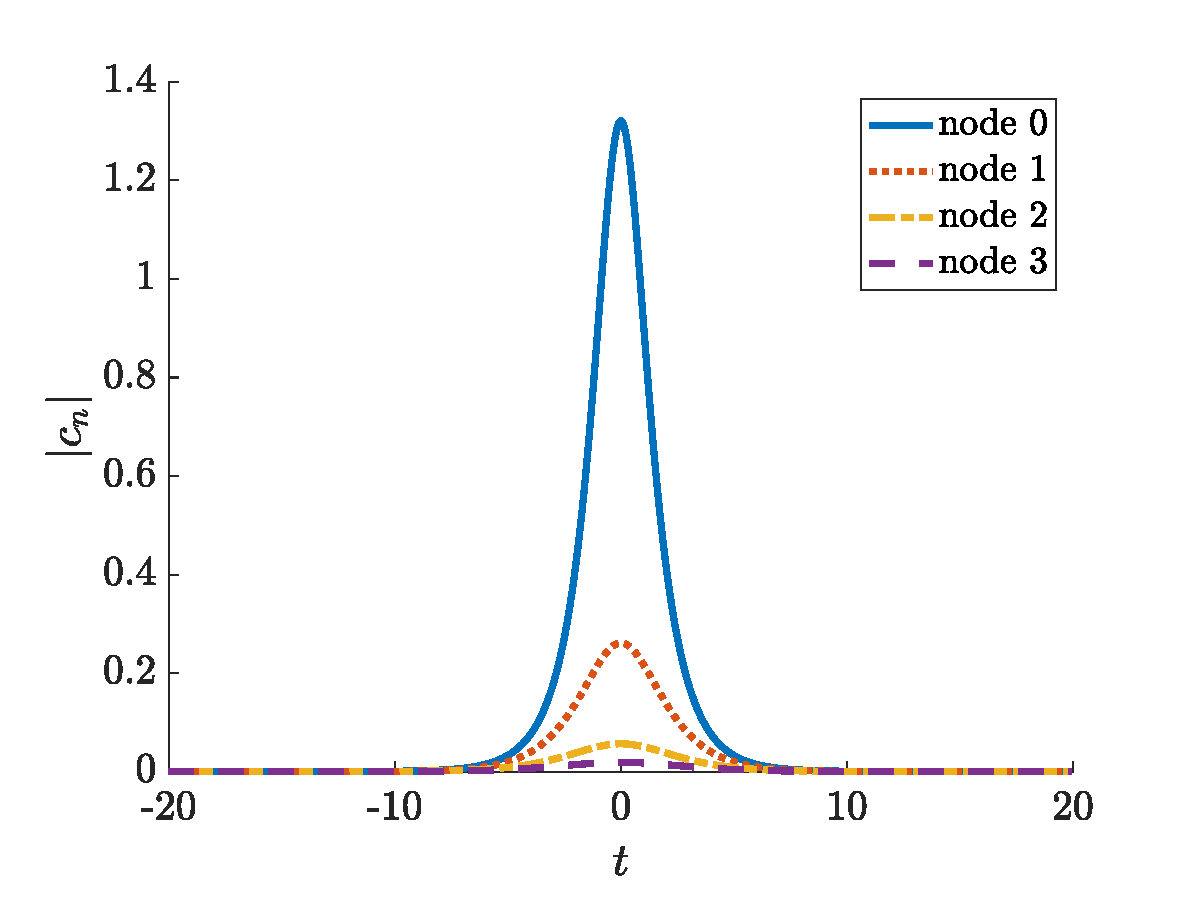
\includegraphics[width=5cm]{m6phi025amp.eps}
    \end{subfigure}
    \begin{subfigure}{0.3\linewidth}
        \caption{}
        \label{fig:m6025logamp}
        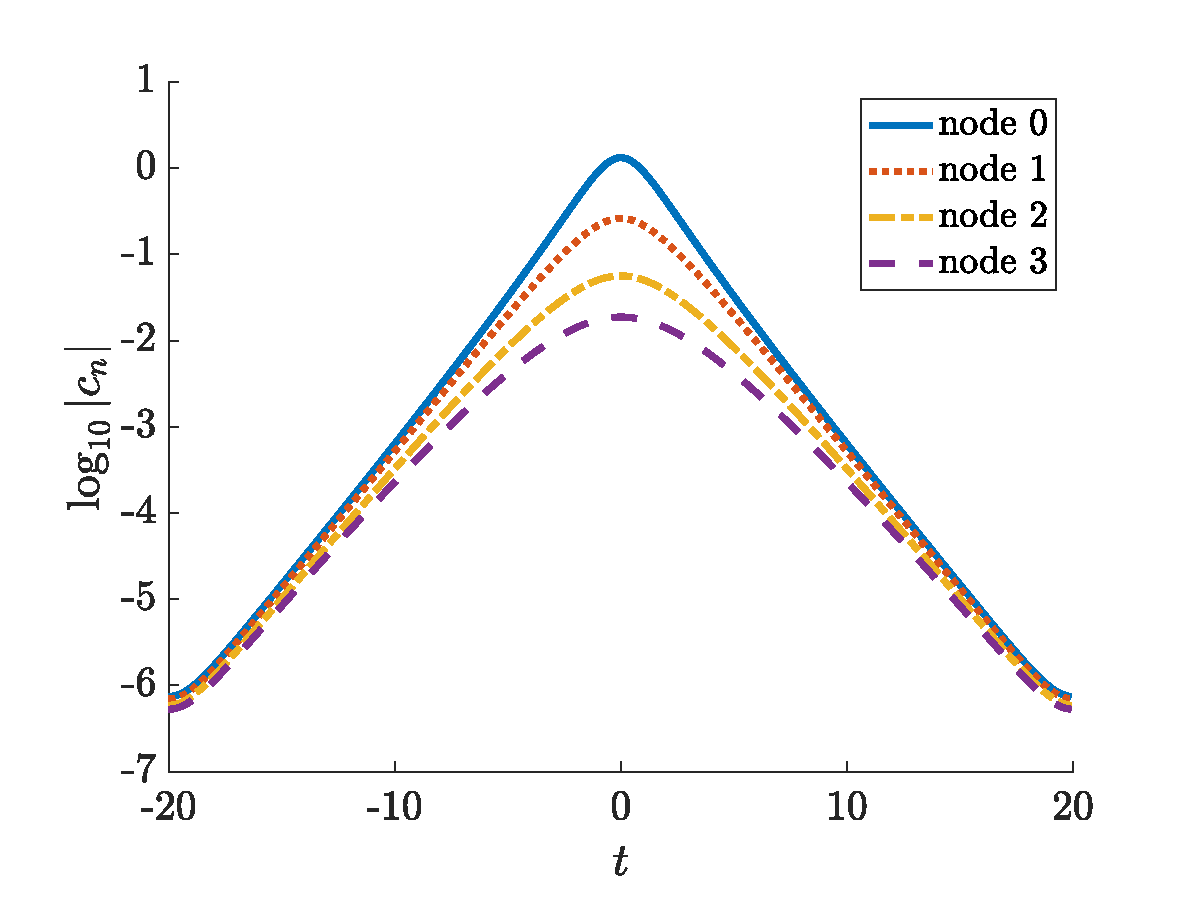
\includegraphics[width=5cm]{m6phi025logamp.eps}
    \end{subfigure}
    \begin{subfigure}{0.3\linewidth}
        \caption{}
        \label{fig:m6025phase}
        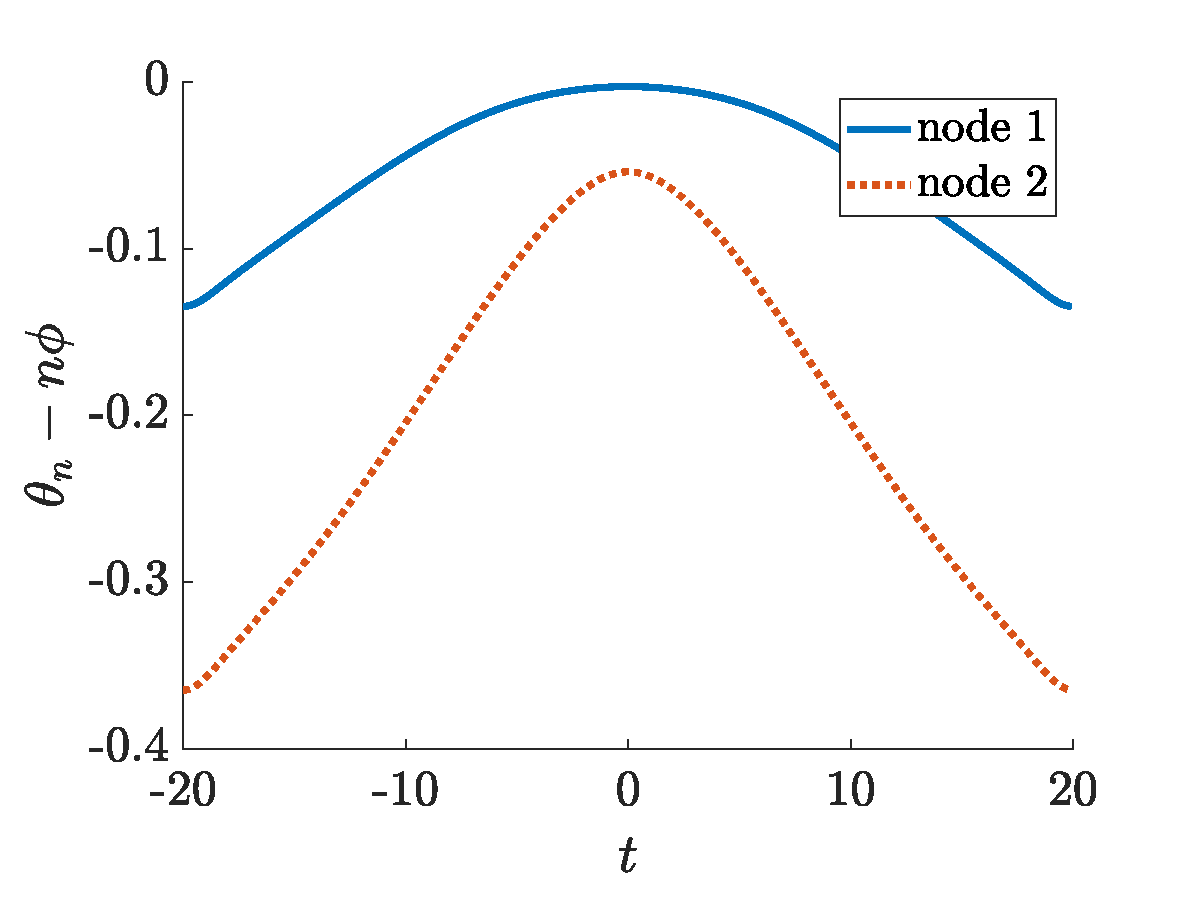
\includegraphics[width=5cm]{m6phi025phase.eps}
    \end{subfigure}
    \begin{subfigure}{0.3\linewidth}
        \caption{}
        \label{fig:m6pi6amp}
        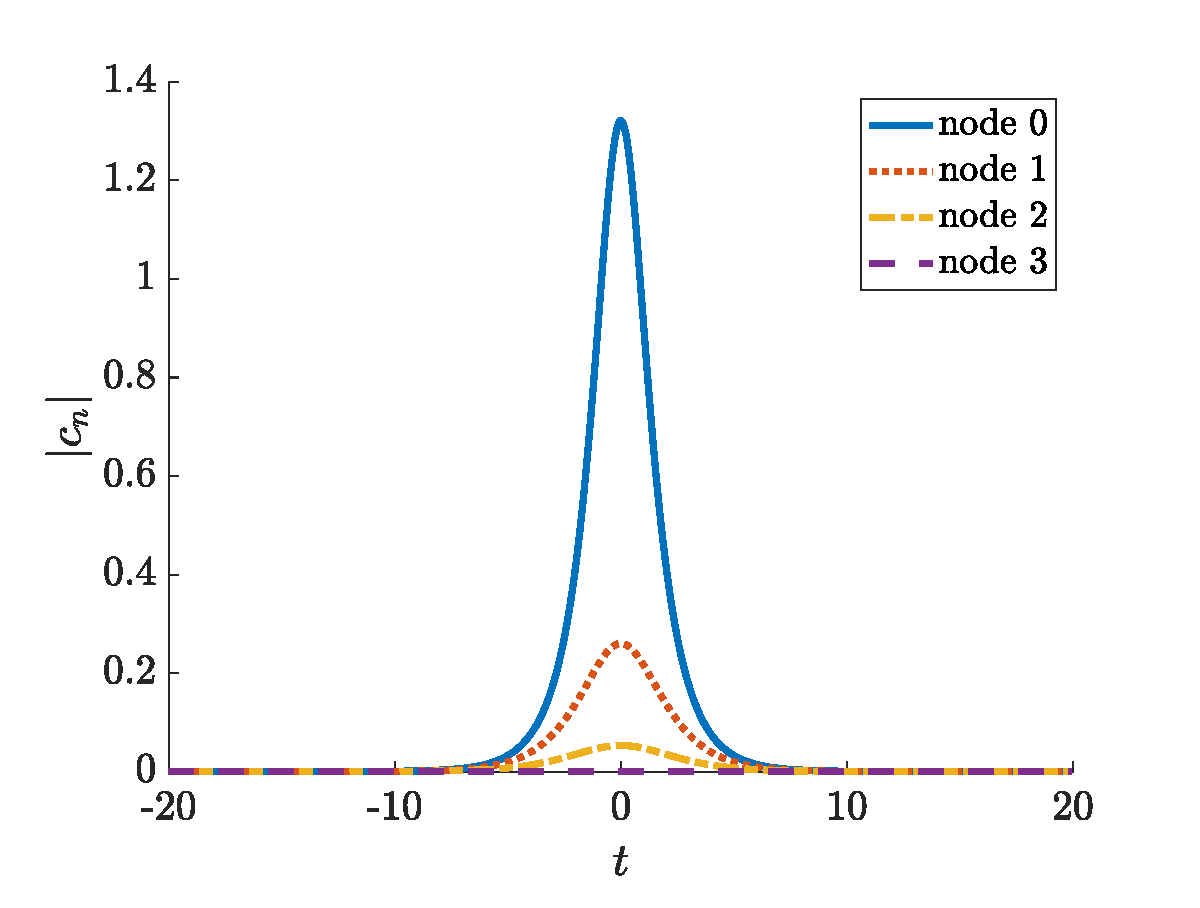
\includegraphics[width=5cm]{m6phipi6amp.eps}
    \end{subfigure}
    \begin{subfigure}{0.3\linewidth}
        \caption{}
        \label{fig:m6pi6logamp}
        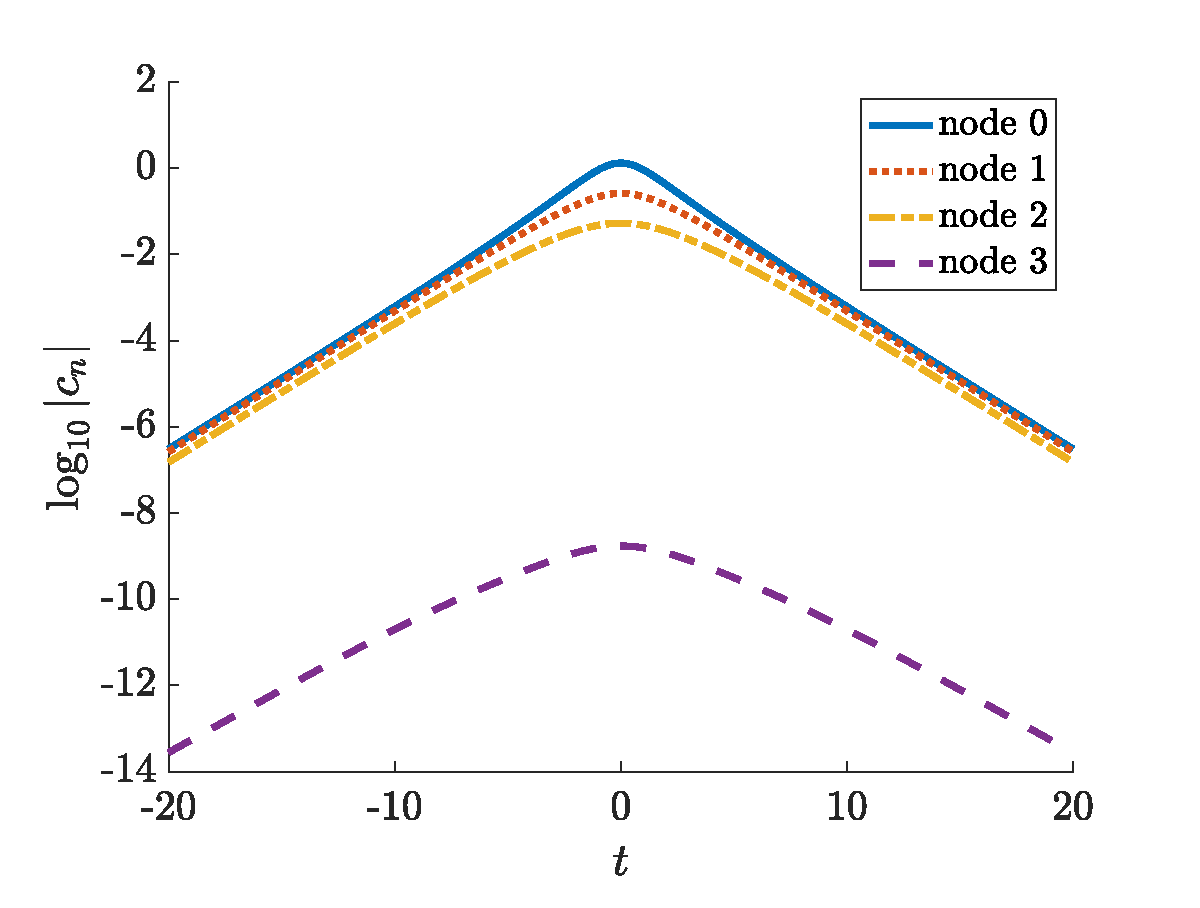
\includegraphics[width=5cm]{m6phipi6logamp.eps}
    \end{subfigure}
        \begin{subfigure}{0.3\linewidth}
        \caption{}
        \label{fig:m6pi6phase}
        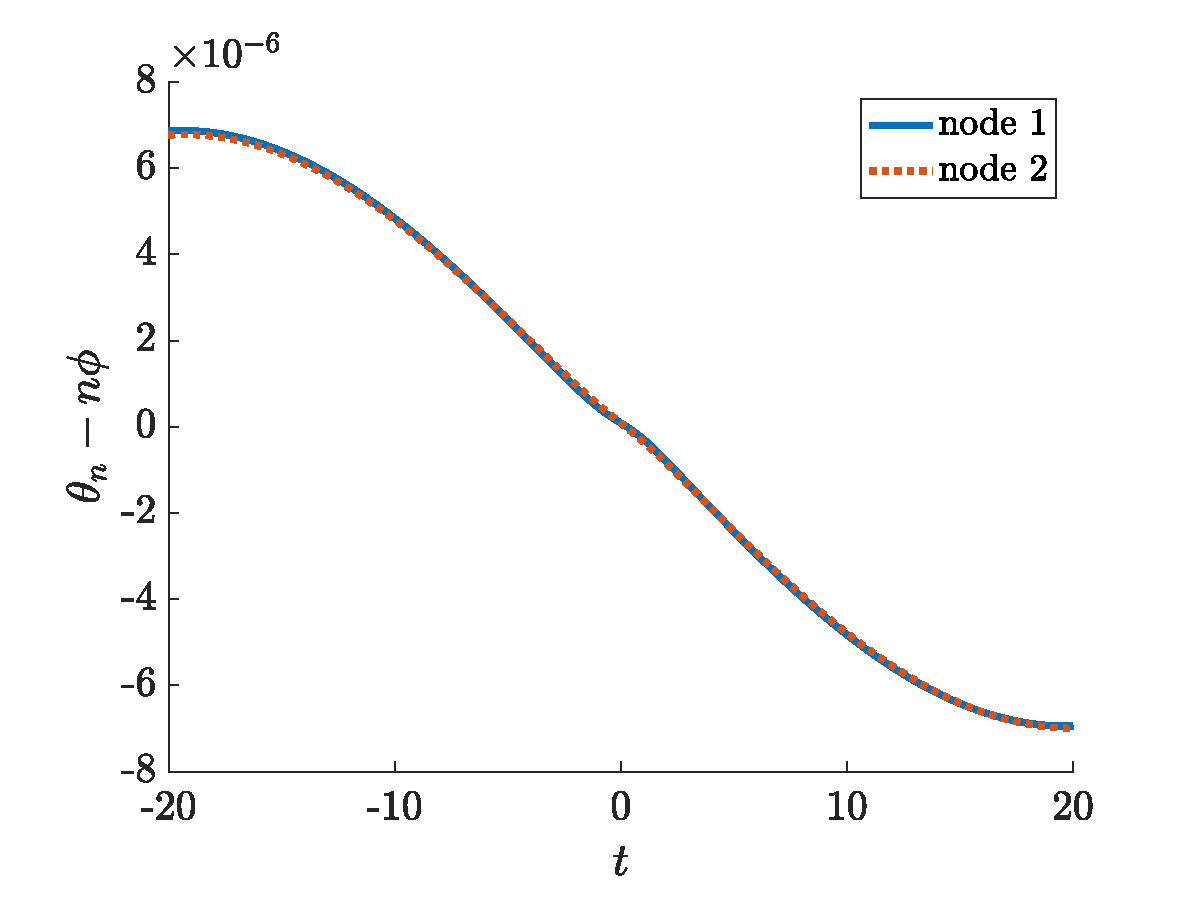
\includegraphics[width=5cm]{m6phipi6phase.eps}
    \end{subfigure}
    \caption{Standing wave solutions to equation \cref{eq:standingwave} for $m=6$ waveguides. Twist parameter $\phi = 0.25$ (top), $\phi = \pi/6$ (bottom). Left and middle are amplitude and log amplitude of solution at first four sites. Right plots $\theta_n(t) - n \phi$ for sites 1 and 2, where $\theta_n(t)$ is the phase. $k=0.25$, $\omega=1$, time domain $[-30,30]$, $N=256$ Fourier nodes.}
    \label{fig:m6sol}
\end{figure}


\appendix

\section{Symmetries}\label{app:symm}

We verify that the symmetry relations in \cref{eq:symm} are consistent. First, for $n = 2, \dots, m/2-1$, we take equation \cref{eq:st2} for $-n$, substitute the symmetries for $a_n$ and $\theta_n$ from \cref{eq:symm}, and simplify, to obtain 
\begin{equation*}
\begin{aligned}
(\ddot a_n &- a_n (\dot \theta_n)^2) 
- i ( a_n \ddot\theta_n + 2 \dot a_n \dot \theta_n )\\
&+ k\left(a_{n-1}e^{i[(\theta_n - \theta_{n-1}) - \phi]} + a_{n+1}e^{-i[(\theta_{n+1} - \theta_{n}) - \phi]} \right)+a_n^3 - \omega a_n = 0,
\end{aligned}
\end{equation*}	
which is the complex conjugate of \cref{eq:st2} for $n$. For $n = 0$, we take equation \cref{eq:st2} for $n=0$, substitute the symmetries for $a_n$ and $\theta_n$ from \cref{eq:symm}, and simplify, to obtain 
\begin{equation*}
\begin{aligned}
(\ddot a_0 &- a_0 (\dot \theta_0)^2) 
+ i ( a_0 \ddot\theta_0 + 2 \dot a_0 \dot \theta_0 )
+ 2 k a_1 \cos(\theta_1 - \phi)(\cos \theta_0 + i \sin \theta_0) + a_n^3 - \omega a_n = 0.
\end{aligned}
\end{equation*}
The imaginary part is
\begin{equation}\label{eq:n0imagpart}
a_0 \ddot\theta_0 + 2 \dot a_0 \dot \theta_0 = 2 k a_1 \cos(\theta_1 - \phi) \sin \theta_0,
\end{equation}
for which $\theta_0(t) = 0$ is a solution, thus this condition is consistent. Following the same procedure by using the imaginary part of equation \cref{eq:st2}, we can show that the $\theta_{m/2} = 0$ is a solution to the imaginary part of \cref{eq:st2} for $n=m/2$, thus this condition is consistent as well.

\section{Asymptotics}\label{app:asymp}

Let $a_m(t)$ and $\theta_m(t)$ be the amplitudes and phases at site $n$, as in the ansatz \cref{eq:cnansatz}, where $n \in S = \{ 0, \pm 1, \dots, \pm m/2-1, m/2 \}$. We will take 
\[
a_m(t), \theta_m(t) \in H^2(\R) \subset L^2(\R),
\]
where $L^2(\R)$ is the space of real, valued square-integrable functions on $\R$ equipped with the standard inner product, and $H^2(\R)$ is the corresponding Sobelev space. We note that the system of equations \cref{eq:st2} is translation invariant, i.e. if $\{ a_n(t), \theta_n(t)\}_{n\in S}$ is a solution, then so is $\{ a_n(t-\tau), \theta_n(t-\tau)\}_{n\in S}$ for any $\tau \in \R$. When $k = 0$, we want the solution $a_0(t)$ to be the ordinary NLS soliton $\psi(t)$, which is centered at 0. To ensure that the solution we find is not shifted in $t$, we impose the phase condition on the amplitude $a_0(t)$
\begin{equation}\label{eq:phasecond}
\langle a_0(t), \dot{\psi}(t) \rangle_{L^2(\R)} = \int_{-\infty}^\infty a_0(t) \dot{\psi}(t) dt = 0.
\end{equation}
In other words, $a_0(t)$ will have no component in the direction of $\dot{\psi}(t)$.

Next, define the linear operator $\Lw: H^2(\R) \subset L^2(\R) \rightarrow L^2(\R)$ by
\begin{equation}\label{eq:Lw}
\Lw = \omega - \partial_t^2.
\end{equation}
Since all functions in $L^2(\R)$ vanish at infinity, the kernel of $\Lw$ is $\{0\}$, i.e. the only solution in $H^2(\R)$ to $\Lw f = 0$ is $f = 0$. Furthermore the operator $\Lw$ is invertible [REF?].

Finally, we recall that the NLS soliton $\psi(t)$ is a real-valued, standing wave solution to the NLS equation with frequency $\omega$, thus it solves 
\begin{equation}\label{eq:NLSreal}
\ddot{u} + u^3 - \omega u = 0. 
\end{equation}
Linearizing this equation about $\dot{\psi}(t)$ yields the self-adjoint linear operator $\calL(\psi): H^2(\R) \subset L^2(\R) \rightarrow L^2(\R)$, defined by
\begin{equation}\label{eq:Lpsi}
\calL(\psi) = \partial_t^2 - \omega + 3 \psi^2.
\end{equation}
The kernel of $\dot{\psi}(t)$ is one-dimensional, and is spanned by $\{ \dot{\psi}(t) \}$. By the Fredholm alternative [REF], since $\calL(\psi)$ is self-adjoint, the equation $\calL(\psi) = u(t)$ has a solution if $u(t) \perp \dot{\psi}(t)$.

\subsection{Node 0}

Using the symmetry relations \cref{eq:symm} and $\theta_0(t) = 0$, equation \cref{eq:st2real} for $n=0$ becomes
\begin{equation}\label{eq:st2reala0}
\ddot a_0  + 2 k a_1 \cos(\theta_1 - \phi) + a_0^3 - \omega a_0 = 0 
\end{equation}
We take the power series ansatz 
\[
a_0(t) = \psi(t) + k a_0^{(1)}(t) + k^2 a_0^{(2)}(t) + \mathcal{O}(k^3)
\]
for the amplitude $a_0(t)$, where $\psi(t)$ is the NLS soliton \cref{eq:NLSsoliton}. In addition, from \cref{eq:basicseries}, we have, at minimum, 
\[
a_1(t) = k \tilde{a}_1(t) + \mathcal{O}(k^2), \qquad \theta_1(t) = \phi + \mathcal{O}(k).
\]
Substituting this into \cref{eq:st2reala0}, using the Taylor series expansion $\cos(\theta_1-\phi) = \mathcal{O}(k^2)$, collecting powers of $k$, and simplifying, we get
\begin{equation*}
\begin{aligned}
&\left(\ddot{\psi} + \psi^3 - \omega \psi\right) 
+ k\left(\ddot a_0^{(1)} - \omega a_0^{(1)} + 3 \psi^2 a_0^{(1)}\right) \\
&\qquad\qquad+ k^2\left(\ddot a_0^{(2)} - \omega a_0^{(2)} + 3\left(a_0^{(1)}\right)^2 + 3 \psi^2 a_0^{(2)} + 2 \tilde{a}_1 \right) + \mathcal{O}(k^3) = 0,
\end{aligned}
\end{equation*}
where we have dropped the dependence on $t$ for simplicity. The $\mathcal{O}(1)$ term is 0 since $\psi$ solves \cref{eq:NLSreal}. The $\mathcal{O}(k)$ term can be written as $\calL(\psi)a_0^{(1)}=0$, where $\calL(\psi)$ is defined by \cref{eq:Lpsi}. Since the kernel of $\calL(\psi)$ is spanned by $\dot \psi(t)$, $a_0^{(1)} = c \dot \psi(t)$ for some constant $c$. However, since we wish our solution to satisfy the phase condition \cref{eq:phasecond}, we will take $c = 0$, from which it follows that $a_0^{(1)} = 0$. The $\mathcal{O}(k^2)$ term then becomes
\[
\ddot a_0^{(2)} - \omega a_0^{(2)} + 3 \psi^2 a_0^{(2)} + 2 \tilde{a}_1 = 0.
\]
Letting $\tilde{a}_0(t) = a_0^{(2)}(t)$, we rewrite this as
\begin{align}\label{eq:solvea0ta}
\calL(\psi) \tilde{a}_0 = -2 \tilde{a}_1.
\end{align}
Once we determine $\tilde{a}_1$, which we will do in the next step, we can solve for $\tilde{a}_0$, provided $\tilde{a}_1 \perp \dot\psi$. Putting all of this together, we have the expression for $a_0$
\begin{equation}\label{eq:a0eq}
a_0(t) = \psi(t) + k^2 \tilde{a}_0(t) + \mathcal{O}(k^3) = \psi(t) + \mathcal{O}(k^2).
\end{equation}

\subsection{Amplitudes}

We can now determine the leading order terms for the amplitudes $a_n$, for $n = 1, \dots, m/2$, using the real parts \cref{eq:st2real} of the equations \cref{eq:st2}. The phases $\theta_n$ will be determined in the next step. For $n=1$, we take the power series ansatz 
\[
a_1(t) = k \tilde{a}_1(t) + \mathcal{O}(k^2).
\]
From \cref{eq:basicseries}, we have, at minimum,
\[
a_2(t) = \mathcal{O}(k^2), \qquad \theta_1(t) = \phi + \mathcal{O}(k), \qquad \theta_2(t) = 2 \phi + \mathcal{O}(k),
\]
and we note that $\dot \theta_1(t) = \mathcal{O}(k)$. Substituting these together with the expression \cref{eq:a0eq} for $a_0(t)$ into the $n=1$ equation of \cref{eq:st2real}, expanding the cosine terms in Taylor series, collecting powers of $k$, and simplifying, we obtain the equation
\[
k\left(\partial_t^2 \tilde{a}_1 - \omega \tilde{a}_1 + \psi\right) + \mathcal{O}(k^2) = 0.
\]
We note that the nonlinear term $a_1^3$ does not contribute to the lowest order term in the asymptotic expansion. We use the $\mathcal{O}(k)$ term to solve for $\tilde{a}_1$ to get 
\begin{equation}\label{eq:a11}
\tilde{a}_1(t) = (\omega - \partial_t^2)^{-1} \psi(t),
\end{equation}
which has a solution since $\Lw$ is invertible. This gives us
\begin{equation}\label{eq:a1eq}
a_1(t) = k (\omega - \partial_t^2) \psi(t) + \mathcal{O}(k^2).
\end{equation}

We continue this process iteratively from $n=2$ to $n=m/2-1$. We take the power series ansatz 
\[
a_n(t) = k^n \tilde{a}_n(t) + \mathcal{O}(k^{n+1}),
\]
and use
\begin{align*}
&a_{n-1}(t) = k^{n-1} \tilde{a}_{n-1}(t) + \mathcal{O}(k^{n}), &&a_{n+1}(t) = \mathcal{O}(k^{n+1}), \\
&\theta_{n-1}(t) = (n-1) \phi + \mathcal{O}(k), &&\theta_{n+1}(t) = (n+1) \phi + \mathcal{O}(k),
\end{align*}
where the expression for $a_{n-1}(t)$ was found in the previous step. Substituting these into \cref{eq:st2real} and following the same procedure as above, we obtain the equation
\begin{align*}
k^n\left(\partial_t^2 \tilde{a}_n - \omega \tilde{a}_n + \tilde{a}_{n-1} \right) +\mathcal{O}(k^{n+1}) = 0.
\end{align*}
We use the $\mathcal{O}(k^n)$ term to solve for $\tilde{a}_n$ to get 
\begin{equation}\label{eq:ann}
\tilde{a}_n = (\omega - \partial_t^2)^{-1}\tilde{a}_{n-1},
\end{equation}
which gives us
\begin{equation}\label{eq:aneq}
a_n(t) = k^n (\omega - \partial_t^2)^{-1} \tilde{a}_{n-1}(t) + \mathcal{O}(k^{n+1}).
\end{equation}
We note that it follows from the ansatz $\theta_n = n \phi + \mathcal{O}(k)$ that $\cos[(\theta_n - \theta_{n-1}) - \phi] = 1 + \mathcal{O}(k^2)$ for all $n$, i.e. all the cosine terms are 1 to leading order. 

For the final node $n=m/2$, we take $\theta_{m/2}(t) = 0$ in the real part of \cref{eq:st2} for $n = m/2$, use the symmetry relations for $a_{m/2-1}$ and $\theta_{m/2-1}$ from \cref{eq:symm}, and simplify to get
\[
\ddot a_{m/2} - a_{m/2} (\dot \theta_{m/2})^2 + 
2 k a_{m/2-1}\cos( \theta_{m/2-1} + \phi) + a_{m/2}^3 - \omega a_{m/2} = 0.
\]
Using the power series ansatz
\[
a_{m/2}(t) = k^{m/2} \tilde{a}_{m/2}(t) + \mathcal{O}(k^{m/2+1})
\]
and the formula $a_{m/2-1}(t) = k^{m/2-1} \tilde{a}_{m/2-1}(t) + \mathcal{O}(k^{m/2})$ from the previous step, we obtain the expression
\begin{equation}\label{eq:am2a}
\tilde{a}_{m/2} = 2 (\omega - \partial_t^2)^{-1}\cos( \theta_{m/2-1} + \phi) \tilde{a}_{m/2-1}.
\end{equation}
It is important to note that since $\theta_{m/2} = 0$, the cosine term in \cref{eq:am2a} is order $\mathcal{O}(1)$. Substituting the ansatz $\theta_{m/2-1}(t) = (m/2-1)\phi + \mathcal{O}(k)$ and simplifying, equation \cref{eq:am2a} becomes
\begin{equation}\label{eq:am2}
\tilde{a}_{m/2} = 2 \cos( m\phi/2)(\omega - \partial_t^2)^{-1} \tilde{a}_{m/2-1} + \mathcal{O}(k).
\end{equation}
Since $\tilde{a}_{m/2} = \mathcal{O}(1)$, it follows that
\begin{equation}\label{eq:am2eq}
a_{m/2}(t) = 2 k^{m/2} \cos\left( m \phi / 2\right) (\omega - \partial_t^2)^{-1} \tilde{a}_{n-1}(t) + \mathcal{O}(k^{m/2}+1).
\end{equation}
Finally, since we have derived an expression \cref{eq:a11} for $\tilde{a}_1$, we substitute this into \cref{eq:solvea0ta} to get 
\[
\calL(\psi) \tilde{a}_0 = -2 (\omega - \partial_t^2)^{-1} \psi(t),
\]
which we can solve for $\tilde{a}_0$.

\subsection{Phases}

Now that we have determined the leading order terms for the amplitudes $a_n(t)$, we will compute the leading order terms for the phases $\theta_n(t)$. In fact, we will get expressions for the products $\tilde{a}_n(t) \tilde{\theta}_n(t)$ of the leading order terms of the amplitudes and the phases. To do this, we will use the imaginary parts \cref{eq:st2imag} of the equations \cref{eq:st2}, this time working backwards from $n = m/2-1$ to $n=1$. (Equations \cref{eq:st2} have already been satisfied for $n=m/2$ and $n=0$ by taking $\theta_{m/2}(t) = 0$ and $\theta_0(t) = 0$, respectively). For $n=m/2-1$, substitute the power series ansatz
\[
\theta_{m/2-1}(t) = k^2 \tilde{\theta}_{m/2-1}(t) + \mathcal{O}(k^{3}),
\]
the expressions for $a_n(t)$ from the previous section, $\theta_m = 0$, and
$\theta_{m/2-2}(t) = (m/2-2)\phi + \mathcal{O}(k^4)$ from \cref{eq:basicseries} into equation \cref{eq:st2} for $n=m/2-1$ to get
\[
k^{m/2+1} \left( \tilde{a}_{m/2-1} \ddot{\tilde{\theta}}_{m/2-1} + 2 \dot{\tilde{a}}_{m/2-1} \dot{\tilde{\theta}}_{m/2-1} - \tilde{a}_{m/2-2} \tilde{\theta}_{m/2-1} - \tilde{a}_{m/2} \sin(m \phi/2) \right) + \mathcal{O}(k^{m/2+2}) = 0.
\]
We use the $\mathcal{O}(k^{m/2+1})$ term to solve for $\tilde{\theta}_{m/2-1}$. First, we solve equation \cref{eq:ann} for $\tilde{a}_{m/2-2}$ and substitute this above to get
\[
\tilde{a}_{m/2-1} \ddot{\tilde{\theta}}_{m/2-1} + 2 \dot{\tilde{a}}_{m/2-1} \dot{\tilde{\theta}}_{m/2-1} - \tilde{\theta}_{m/2-1} (\omega - \partial_t^2) \tilde{a}_{m/2-1} - \tilde{a}_{m/2} \sin(m \phi/2) = 0,
\]
which simplifies as the derivative of a product to get
\[
(\omega - \partial_t^2)\left( \tilde{a}_{m/2-1} \tilde{\theta}_{m/2-1} \right) = -\sin(m \phi/2) \tilde{a}_{m/2}.
\]
Applying $(\omega - \partial_t^2)^{-1}$ to both sides, we obtain the formula
\begin{equation}\label{am2thm2}
\tilde{a}_{m/2-1} \tilde{\theta}_{m/2-1} = -\sin(m \phi/2) (\omega - \partial_t^2)^{-1} \tilde{a}_{m/2},
\end{equation}
and we can divide by $\tilde{a}_{m/2-1}$ to solve for $\tilde{\theta}_{m/2-1}$. Using equation \cref{eq:am2} for $\tilde{a}_{m/2}$, equation \cref{am2thm2} becomes
\[
\tilde{a}_{m/2-1} \tilde{\theta}_{m/2-1} = -2 \sin(m \phi/2) \cos( m\phi/2) (\omega - \partial_t^2)^{-2} \tilde{a}_{m/2-1},
\]
which simplifies to 
\begin{equation}\label{am2thm2a}
\tilde{a}_{m/2-1} \tilde{\theta}_{m/2-1} = -\sin(m \phi) (\omega - \partial_t^2)^{-2} \tilde{a}_{m/2-1}
\end{equation}
using the double angle formula.

We now follow an iterative procedure from $n=m/2-2$ down to $n=1$. For $n$, substitute the power series ansatz
\[
\theta_{n}(t) = k^{m-2n} \tilde{\theta}_{n}(t) + \mathcal{O}(k^{m-2n+1}),
\]
the expressions for $a_n(t)$ from the previous section, and $\theta_n(t)$ from \cref{eq:basicseries} into equation \cref{eq:st2imag} for $n$, and simplify, to get
\[
k^{m/2} \left( \tilde{a}_n \ddot{\tilde{\theta}}_n + 2 \dot{\tilde{a}}_n \dot{\tilde{\theta}}_n
- \tilde{a}_{n-1} \tilde{\theta}_n + \tilde{a}_{n+1}\tilde{\theta}_{n+1} \right) + \mathcal{O}\left(k^{m/2+1}\right) = 0
\]
We use the $\mathcal{O}(k^{m/2})$ term to solve for $\tilde{\theta}_{n}$. First, we solve equation \cref{eq:ann} for $\tilde{a}_{n-1}$ and substitute this above to get
\[
\tilde{a}_n \ddot{\tilde{\theta}}_n + 2 \dot{\tilde{a}}_n \dot{\tilde{\theta}}_n
- \tilde{\theta}_n (\omega - \partial_t^2) \tilde{a}_n + \tilde{a}_{n+1} \tilde{\theta}_{n+1} = 0,
\]
which simplifies as the derivative of a product to get
\[
(\omega - \partial_t^2)\left( \tilde{a}_n \tilde{\theta}_n \right) = \tilde{a}_{n+1} \tilde{\theta}_{n+1}.
\]
Applying $(\omega - \partial_t^2)^{-1}$ to both sides, we obtain the formula
\begin{equation}\label{an2th}
\tilde{a}_n \tilde{\theta}_n = (\omega - \partial_t^2)^{-1} \left( \tilde{a}_{n+1} \tilde{\theta}_{n+1} \right),
\end{equation}
and we can divide by $\tilde{a}_n$ to solve for $\tilde{\theta}_n$. 

\end{document}